
%  article.tex (Version 3.3, released 19 January 2008)
%  Article to demonstrate format for SPIE Proceedings
%  Special instructions are included in this file after the
%  symbol %>>>>
%  Numerous commands are commented out, but included to show how
%  to effect various options, e.g., to print page numbers, etc.
%  This LaTeX source file is composed for LaTeX2e.

%  The following commands have been added in the SPIE class 
%  file (spie.cls) and will not be understood in other classes:
%  \supit{}, \authorinfo{}, \skiplinehalf, \keywords{}
%  The bibliography style file is called spiebib.bst, 
%  which replaces the standard style unstr.bst.  

\documentclass[a4paper]{spie}  %>>> use for US letter paper
%%\documentclass[a4paper]{spie}  %>>> use this instead for A4 paper
%%\documentclass[nocompress]{spie}  %>>> to avoid compression of citations
%% \addtolength{\voffset}{9mm}   %>>> moves text field down
%% \renewcommand{\baselinestretch}{1.65}   %>>> 1.65 for double spacing, 1.25 for 1.5 spacing 
%  The following command loads a graphics package to include images 
%  in the document. It may be necessary to specify a DVI driver option,
%  e.g., [dvips], but that may be inappropriate for some LaTeX 
%  installations. 
\usepackage[]{graphicx}
\usepackage{hyperref}
\usepackage{listings}
\hypersetup{
    colorlinks,
    linkcolor={black!50!black},
    citecolor={blue!50!black},
    urlcolor={blue!80!black}
}
\usepackage{pdfpages}
\usepackage{parcolumns}

\usepackage[utf8]{inputenc} 
\usepackage[english]{babel}

\usepackage{color}
\definecolor{lightgray}{rgb}{.9,.9,.9}
\definecolor{darkgray}{rgb}{.4,.4,.4}
\definecolor{purple}{rgb}{0.65, 0.12, 0.82}

\lstdefinelanguage{JavaScript}{
  keywords={typeof, new, true, false, catch, function, return, null, catch, switch, var, if, in, while, do, else, case, break},
  keywordstyle=\color{blue}\bfseries,
  ndkeywords={class, export, boolean, throw, implements, import, this},
  ndkeywordstyle=\color{darkgray}\bfseries,
  identifierstyle=\color{black},
  sensitive=false,
  comment=[l]{//},
  morecomment=[s]{/*}{*/},
  commentstyle=\color{purple}\ttfamily,
  stringstyle=\color{red}\ttfamily,
  morestring=[b]',
  morestring=[b]"
}

\lstdefinelanguage{JSON}{
  keywords={typeof, new, true, false, catch, function, return, null, catch, switch, var, if, in, while, do, else, case, break},
  keywordstyle=\color{blue}\bfseries,
  ndkeywords={export, boolean, throw, implements, import, this},
  ndkeywordstyle=\color{darkgray}\bfseries,
  identifierstyle=\color{black},
  sensitive=false,
  comment=[l]{//},
  morecomment=[s]{/*}{*/},
  commentstyle=\color{purple}\ttfamily,
  stringstyle=\color{red}\ttfamily,
  morestring=[b]',
  morestring=[b]"
}

\usepackage{array}
\newcolumntype{L}[1]{>{\raggedright\let\newline\\\arraybackslash\hspace{0pt}}m{#1}}
\newcolumntype{C}[1]{>{\centering\let\newline\\\arraybackslash\hspace{0pt}}m{#1}}
\newcolumntype{R}[1]{>{\raggedleft\let\newline\\\arraybackslash\hspace{0pt}}m{#1}}

\usepackage{xcolor,colortbl}
\usepackage{color}
\usepackage{babelbib}


\title{Robot Applications} 

%>>>> The author is responsible for formatting the 
%  author list and their institutions.  Use  \skiplinehalf 
%  to separate author list from addresses and between each address.
%  The correspondence between each author and his/her address
%  can be indicated with a superscript in italics, 
%  which is easily obtained with \supit{}.

\author{Lars Engel, Vikash, Ahsan Yousuf
\\\textit{\\Faculty of Computer Science and Electrical Engineering
\\Fachhochschule Kiel: University of Applied Sciences\\ Kiel, Germany}
}

%%%%%%%%%%%%%%%%%%%%%%%%%%%%%%%%%%%%%%%%%%%%%%%%%%%%%%%%%%%%% 
%>>>> uncomment following for page numbers
   
%>>>> uncomment following to start page numbering at 301 
%\setcounter{page}{301} 

\date{\today}  
 
  \begin{document} 
  
  \begin{LARGE}
  \maketitle
  \end{LARGE}
  \vspace{60pt}
  \begin{large}
  \tableofcontents
  \newpage

%%%%%%%%%%%%%%%%%%%%%%%%%%%%%%%%%%%%%%%%%%%%%%%%%%%%%%%%%%%%% 
\pagestyle{plain} 
\setcounter{page}{1}

\section{Introduction}
Just a short introduction for motivation of project (why should we let the robot play this game?)
\section{Background}
\subsection{Explanation and Description of Robot}
\subsection{Explanation and Description of Camera}
\subsection{Explanation and Description of Ninemens Morris}
\subsection{Explanation and Description of the AI}
\section{Implementation}

\subsection{Description of Classes}
\subsubsection{RobotInteractions}
\begin{figure}[h]
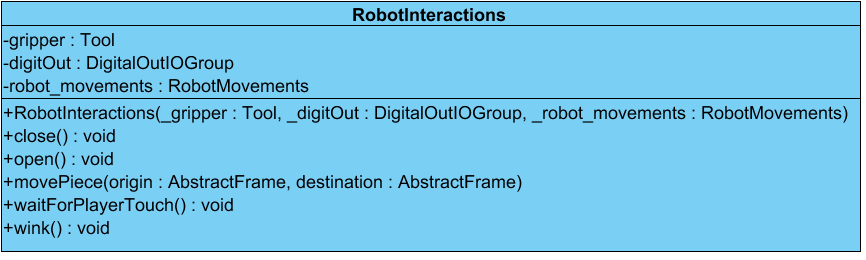
\includegraphics[width=15cm]{images/class_roboInt.png}
\centering
\caption{Class diagram of the RobotInteractions class}
\end{figure}
\subsubsection{RobotMovements}
\begin{figure}[h]
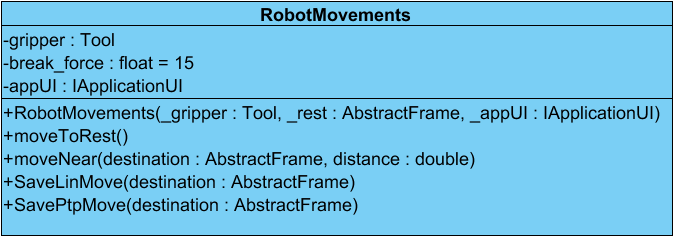
\includegraphics[width=12cm]{images/class_roboMov.png}
\centering
\caption{Class diagram of the RobotMovements class}
\end{figure}
\subsubsection{Bordpoints}
\begin{figure}[h]
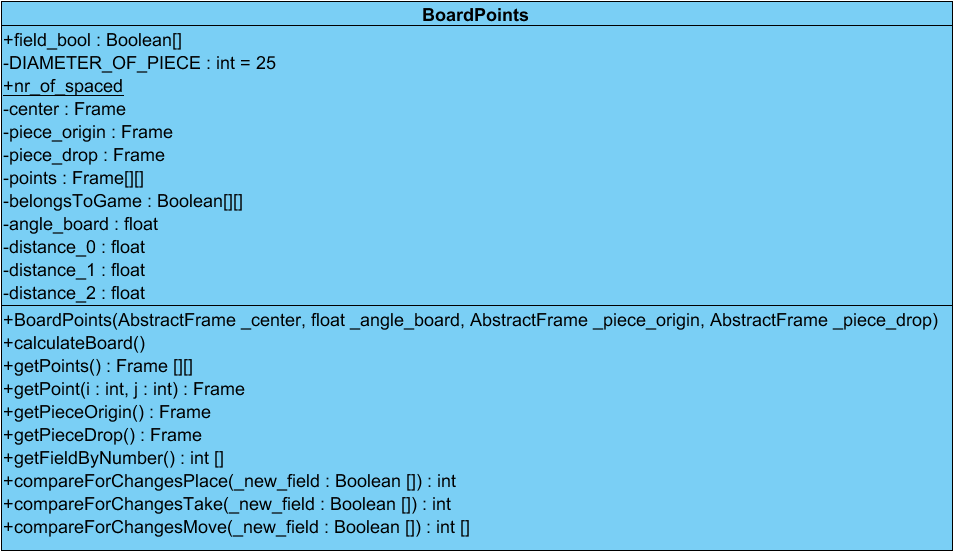
\includegraphics[width=15cm]{images/class_boPo.png}
\centering
\caption{Class diagram of the BoardPoints class}
\end{figure}
\subsubsection{Logger}
\begin{figure}[h]
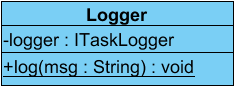
\includegraphics[width=4cm]{images/class_lo.png}
\centering
\caption{Class diagram of the Logger class}
\end{figure}
\subsubsection{ModbusClient}
\begin{figure}[h]
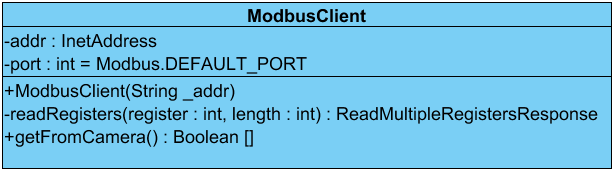
\includegraphics[width=12cm]{images/class_moCli.png}
\centering
\caption{Class diagram of the ModbusClient class}
\end{figure}
\subsection{How did we use the ai?}
\subsubsection{Changes in GameController}
\subsection{How did we use the camera?}
\subsubsection{In-Sight Explorer}
\subsubsection{Communication between Robot and Camera}
\begin{figure}[h]
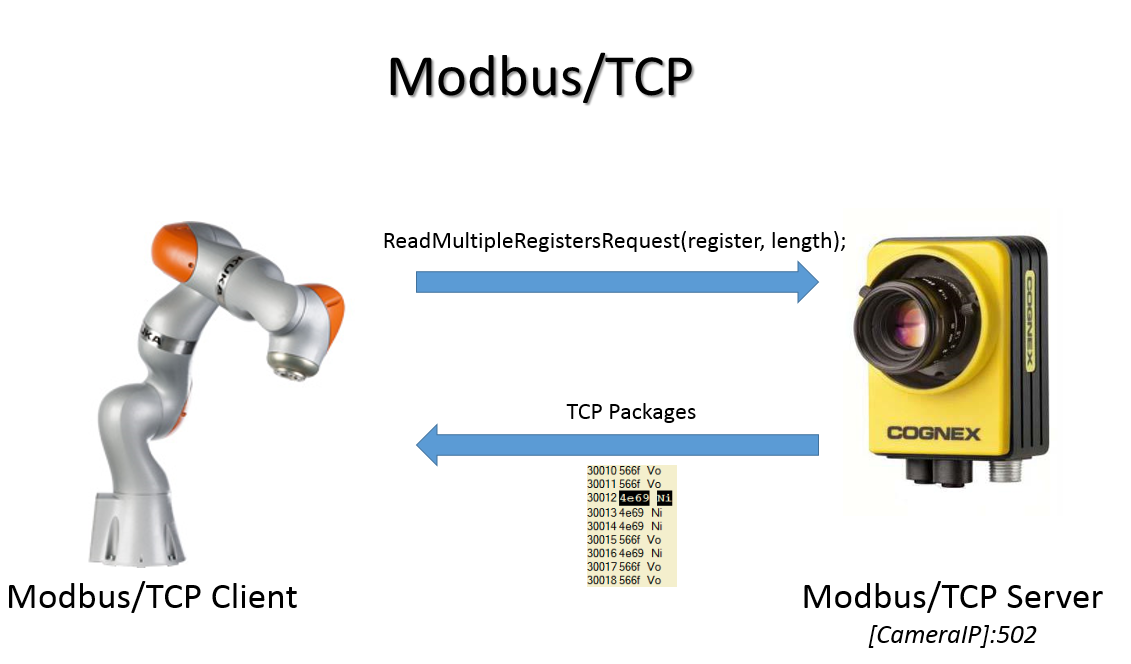
\includegraphics[width=15cm]{images/communication.png}
\centering
\caption{Communication between Camera and Robot}
\end{figure}
\section{Evaluation}
Not sure if we need this or what we should write here...
\section{Conclusion and Future work}
\end{large}
\newpage

%%%%%%%%%%%%%%%%%%%%%%%%%%%%%%%%%%%%%%%%%%%%%%%%%%%%%%%%%%%%%
%%%%% References %%%%%
\bibliographystyle{babunsrt-lf}
%\bibliographystyle{spiebib}   %>>>> makes bibtex use spiebib.bst
\bibliography{references}   %>>>> bibliography data in report.bib


\end{document} 
